\documentclass{extbook}[14pt]
\usepackage{multicol, enumerate, enumitem, hyperref, color, soul, setspace, parskip, fancyhdr, amssymb, amsthm, amsmath, bbm, latexsym, units, mathtools}
\everymath{\displaystyle}
\usepackage[headsep=0.5cm,headheight=0cm, left=1 in,right= 1 in,top= 1 in,bottom= 1 in]{geometry}
\usepackage{dashrule}  % Package to use the command below to create lines between items
\newcommand{\litem}[1]{\item #1

\rule{\textwidth}{0.4pt}}
\pagestyle{fancy}
\lhead{}
\chead{Answer Key for Progress Quiz 8 Version A}
\rhead{}
\lfoot{4553-3922}
\cfoot{}
\rfoot{Fall 2020}
\begin{document}
\textbf{This key should allow you to understand why you choose the option you did (beyond just getting a question right or wrong). \href{https://xronos.clas.ufl.edu/mac1105spring2020/courseDescriptionAndMisc/Exams/LearningFromResults}{More instructions on how to use this key can be found here}.}

\textbf{If you have a suggestion to make the keys better, \href{https://forms.gle/CZkbZmPbC9XALEE88}{please fill out the short survey here}.}

\textit{Note: This key is auto-generated and may contain issues and/or errors. The keys are reviewed after each exam to ensure grading is done accurately. If there are issues (like duplicate options), they are noted in the offline gradebook. The keys are a work-in-progress to give students as many resources to improve as possible.}

\rule{\textwidth}{0.4pt}

\begin{enumerate}\litem{
Describe the end behavior of the polynomial below.
\[ f(x) = 3(x - 5)^{5}(x + 5)^{10}(x + 2)^{2}(x - 2)^{4} \]

The solution is the graph below, which is option D.
\begin{center}
    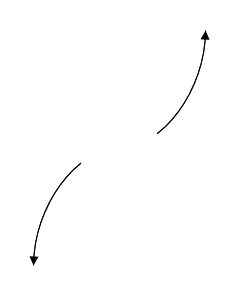
\includegraphics[width=0.3\textwidth]{../Figures/polyEndBehaviorDA.png}
\end{center}\begin{enumerate}[label=\Alph*.]
\begin{multicols}{2}
\item 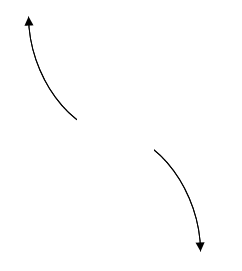
\includegraphics[width = 0.3\textwidth]{../Figures/polyEndBehaviorAA.png}
\item 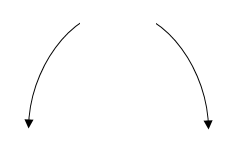
\includegraphics[width = 0.3\textwidth]{../Figures/polyEndBehaviorBA.png}
\item 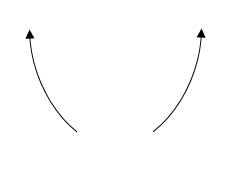
\includegraphics[width = 0.3\textwidth]{../Figures/polyEndBehaviorCA.png}
\item 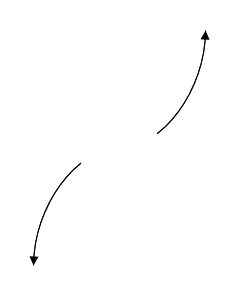
\includegraphics[width = 0.3\textwidth]{../Figures/polyEndBehaviorDA.png}
\end{multicols}\item None of the above.\end{enumerate}
\textbf{General Comment:} Remember that end behavior is determined by the leading coefficient AND whether the \textbf{sum} of the multiplicities is positive or negative.
}
\litem{
Construct the lowest-degree polynomial given the zeros below. Then, choose the intervals that contain the coefficients of the polynomial in the form $ax^3+bx^2+cx+d$.
\[ 2, \frac{7}{5}, \text{ and } \frac{-7}{4} \]

The solution is \( 20x^{3} -33 x^{2} -63 x + 98 \), which is option D.\begin{enumerate}[label=\Alph*.]
\item \( a \in [16, 26], b \in [99, 104], c \in [169, 183], \text{ and } d \in [92, 109] \)

$20x^{3} +103 x^{2} +175 x + 98$, which corresponds to multiplying out $(x + 1)(5x + 5)(4x -4)$.
\item \( a \in [16, 26], b \in [30, 36], c \in [-66, -61], \text{ and } d \in [-98, -94] \)

$20x^{3} +33 x^{2} -63 x -98$, which corresponds to multiplying out $(x + 2)(5x + 7)(4x -7)$.
\item \( a \in [16, 26], b \in [43, 48], c \in [-40, -34], \text{ and } d \in [-98, -94] \)

$20x^{3} +47 x^{2} -35 x -98$, which corresponds to multiplying out $(x + 1)(5x -5)(4x -4)$.
\item \( a \in [16, 26], b \in [-44, -31], c \in [-66, -61], \text{ and } d \in [92, 109] \)

* $20x^{3} -33 x^{2} -63 x + 98$, which is the correct option.
\item \( a \in [16, 26], b \in [-44, -31], c \in [-66, -61], \text{ and } d \in [-98, -94] \)

$20x^{3} -33 x^{2} -63 x -98$, which corresponds to multiplying everything correctly except the constant term.
\end{enumerate}

\textbf{General Comment:} To construct the lowest-degree polynomial, you want to multiply out $(x -2)(5x -7)(4x + 7)$
}
\litem{
Describe the zero behavior of the zero $x = -2$ of the polynomial below.
\[ f(x) = 7(x - 6)^{11}(x + 6)^{8}(x - 2)^{4}(x + 2)^{3} \]

The solution is the graph below, which is option A.
\begin{center}
    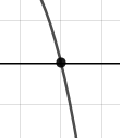
\includegraphics[width=0.3\textwidth]{../Figures/polyZeroBehaviorCopyAA.png}
\end{center}\begin{enumerate}[label=\Alph*.]
\begin{multicols}{2}
\item 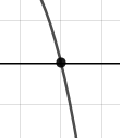
\includegraphics[width = 0.3\textwidth]{../Figures/polyZeroBehaviorCopyAA.png}
\item 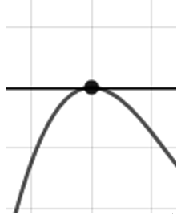
\includegraphics[width = 0.3\textwidth]{../Figures/polyZeroBehaviorCopyBA.png}
\item 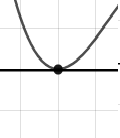
\includegraphics[width = 0.3\textwidth]{../Figures/polyZeroBehaviorCopyCA.png}
\item 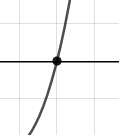
\includegraphics[width = 0.3\textwidth]{../Figures/polyZeroBehaviorCopyDA.png}
\end{multicols}\item None of the above.\end{enumerate}
\textbf{General Comment:} You will need to sketch the entire graph, then zoom in on the zero the question asks about.
}
\litem{
Construct the lowest-degree polynomial given the zeros below. Then, choose the intervals that contain the coefficients of the polynomial in the form $x^3+bx^2+cx+d$.
\[ -3 - 5 i \text{ and } 2 \]

The solution is \( x^{3} +4 x^{2} +22 x -68 \), which is option D.\begin{enumerate}[label=\Alph*.]
\item \( b \in [0.5, 3.6], c \in [1.5, 3.3], \text{ and } d \in [-13, -9] \)

$x^{3} + x^{2} +3 x -10$, which corresponds to multiplying out $(x + 5)(x -2)$.
\item \( b \in [-4.5, -1.5], c \in [17.2, 24.6], \text{ and } d \in [67, 70] \)

$x^{3} -4 x^{2} +22 x + 68$, which corresponds to multiplying out $(x-(-3 - 5 i))(x-(-3 + 5 i))(x + 2)$.
\item \( b \in [0.5, 3.6], c \in [-0.3, 2.4], \text{ and } d \in [-8, 2] \)

$x^{3} + x^{2} +x -6$, which corresponds to multiplying out $(x + 3)(x -2)$.
\item \( b \in [3.9, 4.8], c \in [17.2, 24.6], \text{ and } d \in [-74, -62] \)

* $x^{3} +4 x^{2} +22 x -68$, which is the correct option.
\item \( \text{None of the above.} \)

This corresponds to making an unanticipated error or not understanding how to use nonreal complex numbers to create the lowest-degree polynomial. If you chose this and are not sure what you did wrong, please contact the coordinator for help.
\end{enumerate}

\textbf{General Comment:} Remember that the conjugate of $a+bi$ is $a-bi$. Since these zeros always come in pairs, we need to multiply out $(x-(-3 - 5 i))(x-(-3 + 5 i))(x-(2))$.
}
\litem{
Which of the following equations \textit{could} be of the graph presented below?

\begin{center}
    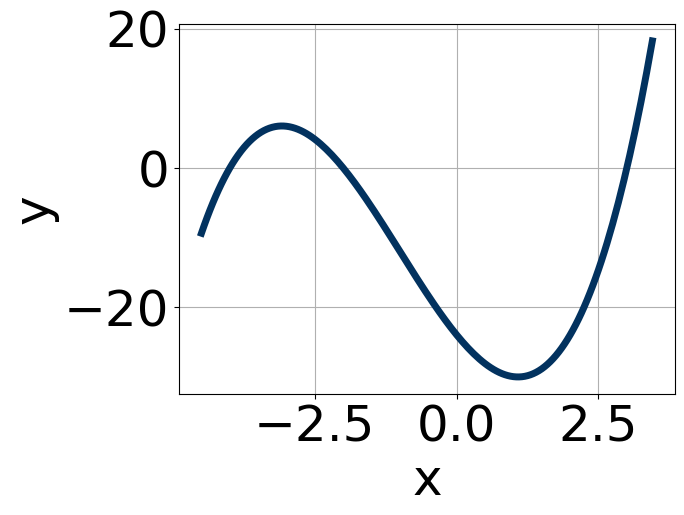
\includegraphics[width=0.5\textwidth]{../Figures/polyGraphToFunctionCopyA.png}
\end{center}




The solution is \( 7x^{9} (x + 2)^{10} (x + 3)^{10} \), which is option C.\begin{enumerate}[label=\Alph*.]
\item \( -15x^{8} (x + 2)^{6} (x + 3)^{6} \)

The factor $x$ should have an odd power and the leading coefficient should be the opposite sign.
\item \( -16x^{7} (x + 2)^{6} (x + 3)^{10} \)

This corresponds to the leading coefficient being the opposite value than it should be.
\item \( 7x^{9} (x + 2)^{10} (x + 3)^{10} \)

* This is the correct option.
\item \( 9x^{8} (x + 2)^{6} (x + 3)^{9} \)

The factor $(x + 3)$ should have an even power and the factor $x$ should have an odd power.
\item \( 15x^{9} (x + 2)^{6} (x + 3)^{5} \)

The factor $(x + 3)$ should have an even power.
\end{enumerate}

\textbf{General Comment:} General Comments: Draw the x-axis to determine which zeros are touching (and so have even multiplicity) or cross (and have odd multiplicity).
}
\litem{
Describe the zero behavior of the zero $x = 7$ of the polynomial below.
\[ f(x) = 2(x - 7)^{9}(x + 7)^{14}(x - 8)^{8}(x + 8)^{11} \]

The solution is the graph below, which is option D.
\begin{center}
    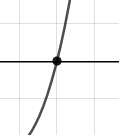
\includegraphics[width=0.3\textwidth]{../Figures/polyZeroBehaviorDA.png}
\end{center}\begin{enumerate}[label=\Alph*.]
\begin{multicols}{2}
\item 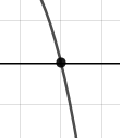
\includegraphics[width = 0.3\textwidth]{../Figures/polyZeroBehaviorAA.png}
\item 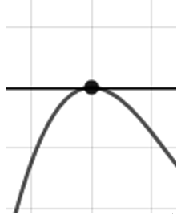
\includegraphics[width = 0.3\textwidth]{../Figures/polyZeroBehaviorBA.png}
\item 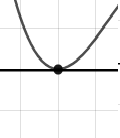
\includegraphics[width = 0.3\textwidth]{../Figures/polyZeroBehaviorCA.png}
\item 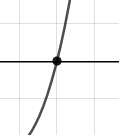
\includegraphics[width = 0.3\textwidth]{../Figures/polyZeroBehaviorDA.png}
\end{multicols}\item None of the above.\end{enumerate}
\textbf{General Comment:} You will need to sketch the entire graph, then zoom in on the zero the question asks about.
}
\litem{
Describe the end behavior of the polynomial below.
\[ f(x) = 8(x - 5)^{3}(x + 5)^{4}(x - 9)^{4}(x + 9)^{4} \]

The solution is the graph below, which is option D.
\begin{center}
    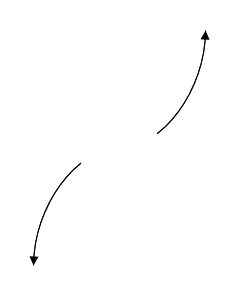
\includegraphics[width=0.3\textwidth]{../Figures/polyEndBehaviorCopyDA.png}
\end{center}\begin{enumerate}[label=\Alph*.]
\begin{multicols}{2}
\item 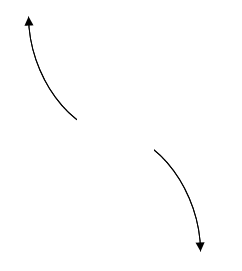
\includegraphics[width = 0.3\textwidth]{../Figures/polyEndBehaviorCopyAA.png}
\item 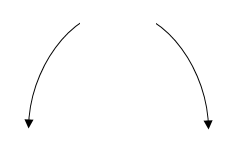
\includegraphics[width = 0.3\textwidth]{../Figures/polyEndBehaviorCopyBA.png}
\item 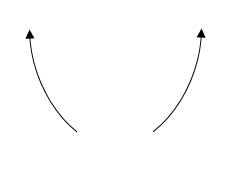
\includegraphics[width = 0.3\textwidth]{../Figures/polyEndBehaviorCopyCA.png}
\item 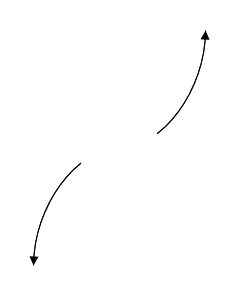
\includegraphics[width = 0.3\textwidth]{../Figures/polyEndBehaviorCopyDA.png}
\end{multicols}\item None of the above.\end{enumerate}
\textbf{General Comment:} Remember that end behavior is determined by the leading coefficient AND whether the \textbf{sum} of the multiplicities is positive or negative.
}
\litem{
Construct the lowest-degree polynomial given the zeros below. Then, choose the intervals that contain the coefficients of the polynomial in the form $x^3+bx^2+cx+d$.
\[ 5 - 2 i \text{ and } 3 \]

The solution is \( x^{3} -13 x^{2} +59 x -87 \), which is option B.\begin{enumerate}[label=\Alph*.]
\item \( b \in [-5, 5], c \in [-10, -7], \text{ and } d \in [10, 18] \)

$x^{3} + x^{2} -8 x + 15$, which corresponds to multiplying out $(x -5)(x -3)$.
\item \( b \in [-19, -8], c \in [57, 68], \text{ and } d \in [-88, -85] \)

* $x^{3} -13 x^{2} +59 x -87$, which is the correct option.
\item \( b \in [-5, 5], c \in [-1, 0], \text{ and } d \in [-14, 2] \)

$x^{3} + x^{2} -x -6$, which corresponds to multiplying out $(x + 2)(x -3)$.
\item \( b \in [13, 15], c \in [57, 68], \text{ and } d \in [82, 95] \)

$x^{3} +13 x^{2} +59 x + 87$, which corresponds to multiplying out $(x-(5 - 2 i))(x-(5 + 2 i))(x + 3)$.
\item \( \text{None of the above.} \)

This corresponds to making an unanticipated error or not understanding how to use nonreal complex numbers to create the lowest-degree polynomial. If you chose this and are not sure what you did wrong, please contact the coordinator for help.
\end{enumerate}

\textbf{General Comment:} Remember that the conjugate of $a+bi$ is $a-bi$. Since these zeros always come in pairs, we need to multiply out $(x-(5 - 2 i))(x-(5 + 2 i))(x-(3))$.
}
\litem{
Construct the lowest-degree polynomial given the zeros below. Then, choose the intervals that contain the coefficients of the polynomial in the form $ax^3+bx^2+cx+d$.
\[ \frac{-2}{5}, \frac{4}{5}, \text{ and } \frac{-3}{2} \]

The solution is \( 50x^{3} +55 x^{2} -46 x -24 \), which is option A.\begin{enumerate}[label=\Alph*.]
\item \( a \in [48, 53], b \in [51, 63], c \in [-47, -44], \text{ and } d \in [-25, -20] \)

* $50x^{3} +55 x^{2} -46 x -24$, which is the correct option.
\item \( a \in [48, 53], b \in [15, 17], c \in [-76, -71], \text{ and } d \in [20, 33] \)

$50x^{3} +15 x^{2} -74 x + 24$, which corresponds to multiplying out $(5x + 5)(5x -5)(2x -2)$.
\item \( a \in [48, 53], b \in [94, 96], c \in [10, 19], \text{ and } d \in [-25, -20] \)

$50x^{3} +95 x^{2} +14 x -24$, which corresponds to multiplying out $(5x + 5)(5x + 5)(2x -2)$.
\item \( a \in [48, 53], b \in [-61, -54], c \in [-47, -44], \text{ and } d \in [20, 33] \)

$50x^{3} -55 x^{2} -46 x + 24$, which corresponds to multiplying out $(5x -2)(5x + 4)(2x -3)$.
\item \( a \in [48, 53], b \in [51, 63], c \in [-47, -44], \text{ and } d \in [20, 33] \)

$50x^{3} +55 x^{2} -46 x + 24$, which corresponds to multiplying everything correctly except the constant term.
\end{enumerate}

\textbf{General Comment:} To construct the lowest-degree polynomial, you want to multiply out $(5x + 2)(5x -4)(2x + 3)$
}
\litem{
Which of the following equations \textit{could} be of the graph presented below?

\begin{center}
    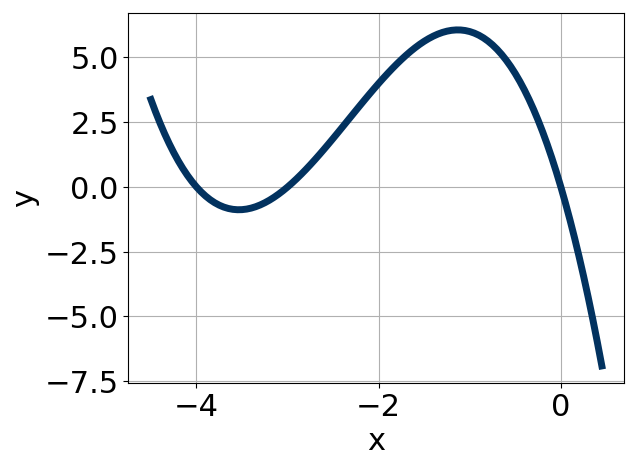
\includegraphics[width=0.5\textwidth]{../Figures/polyGraphToFunctionA.png}
\end{center}




The solution is \( -14(x - 2)^{9} (x + 2)^{7} (x + 1)^{11} \), which is option A.\begin{enumerate}[label=\Alph*.]
\item \( -14(x - 2)^{9} (x + 2)^{7} (x + 1)^{11} \)

* This is the correct option.
\item \( -15(x - 2)^{10} (x + 2)^{8} (x + 1)^{7} \)

The factors $2$ and $-2$ have have been odd power.
\item \( -9(x - 2)^{6} (x + 2)^{7} (x + 1)^{9} \)

The factor $2$ should have been an odd power.
\item \( 18(x - 2)^{10} (x + 2)^{9} (x + 1)^{9} \)

The factor $(x - 2)$ should have an odd power and the leading coefficient should be the opposite sign.
\item \( 19(x - 2)^{5} (x + 2)^{5} (x + 1)^{11} \)

This corresponds to the leading coefficient being the opposite value than it should be.
\end{enumerate}

\textbf{General Comment:} General Comments: Draw the x-axis to determine which zeros are touching (and so have even multiplicity) or cross (and have odd multiplicity).
}
\end{enumerate}

\end{document}